\section{Bartłomiej Mazgaj}
\setlength{\parindent}{20pt}


\textbf{Zdzisław Beksiński} was a Polish painter, photographer, and sculptor; specializing in the field of dystopian surrealism.\par
\textbf{Beksiński} made his paintings and drawings in what he called either a Baroque or a Gothic manner. His creations were made mainly in two periods. The first period of work is generally considered to contain expressionistic color, with a strong style of "utopian realism" and surreal architecture, like a doomsday scenario. The second period contained more abstract style, with the main features of formalism.\par
\textbf{Beksiński} was stabbed to death at his Warsaw apartment on February 21, 2005, by a 19-year-old acquaintance from Wołomin, reportedly because he refused to lend him money. 

\vspace{5mm}
This is a Zdzisław Beksiński's painting (see Figure~\ref{fig:beksinski}).

\begin{figure}[htbp] 
    \centering
    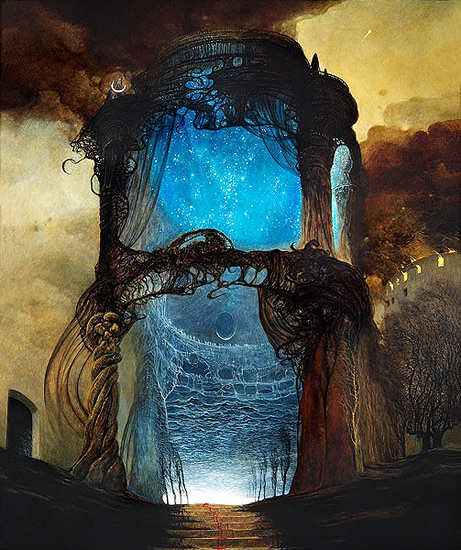
\includegraphics[width=0.4\textwidth]{pictures/Beksinski.jpg} 
    \caption{This painting is mysterious.}
    \label{fig:beksinski}
\end{figure}

Table~\ref{tab:logical_puzzle} is a logic puzzle. 
\begin{table}[htbp]
\centering
\begin{tabular}{|c|c|c|c|}
\hline
\rowcolor[HTML]{67FD9A} 
\textbf{Number 1.} & \textbf{Number 2.} & \textbf{Number 3.} & \textbf{Number 4.} \\ \hline
5                  & 35                 & -56                & -66248             \\
7                  & ?                  & 65                 & 3380               \\
13                 & 26                 & ?                  & ?                  \\
2                  & 10                 & -25                & 6125               \\ \hline
\end{tabular}
\label{tab:logical_puzzle}
\end{table}

Euler's number: \[ lim_{n \to \infty }\left ( 1+\frac{1}{n} \right )^{n}= e \]
\newpage 
Funny names of Beksiński's paintings (list 1.):

\begin{itemize}
    \item    painting AE78
    \item[?] painting AA79
    \item[!] painting C2
\end{itemize}

\vspace{5mm}

Funny names of Beksiński's paintings (list 2.):
\begin{enumerate}
    \item Untitled
    \item Untitled
    \item Untitled
    \item Untitled
    \item Untitled
\end{enumerate}

    
   
   
  


